\documentclass{article}
% Packages
\usepackage{graphicx,subfig,float} % Required for inserting images
\usepackage{changepage}
\usepackage{amsmath}
\usepackage{datetime}
\usepackage[spanish]{babel}
\usepackage{titling}
\usepackage{geometry}

\geometry{
  a4paper,
  total={170mm,257mm},
  width=150mm,
  height=230mm,
}

\usepackage{tcolorbox}

\graphicspath{{assets/}}

\numberwithin{equation}{section}
\renewcommand{\theequation}{\arabic{section}.\arabic{equation}}

\newenvironment{subs}
  {\adjustwidth{3em}{0pt}}
  {\endadjustwidth}

\providecommand{\abs}[1]{\lvert#1\rvert}


\title{Apuntes \\ Conceptos de Arquitectura de Computadoras}
\author{Polanis, Iván Valentín}

\begin{document}

\maketitle

\newpage
\tableofcontents
\newpage

%RESUMEN
\section{Introducción a la Arquitectura de Computadoras}

Cuando se describe un computador, frecuentemente se distingue entre \textit{arquitectura} y \textit{organización}.

La \textit{arquitectura} de computadoras se refiere a los atributos de un sistema que son visibles a un programador, o para decirlo de otra manera,aquellos atributos que tiene un impacto directo en la ejecución lógica de un programa.
En cambio, la \textit{organización} de computadores se refiere a las unidades funcionales y sus interconexiones, que dan lugar a especificaciones arquitectónicas.

\subsection{Arquitectura Von Neumann}

La tarea de cargar y modificar programas para el ENIAC\footnote{Electronic Numerical Integrator And Computer, diseñado y contruido bajo la supervisión de John Mauchly y John Presper Eckert en la Universidad de Pennsylvania, fue el primer computador electrónico de propósito general del mundo.} era extremadamente tediosa. El proceso de programación podría ser más fácil si el programa se representara en una forma adecuada parta ser guardado en la memoria junto con los datos.
Esta idea conocida como \textit{concepto de programa-almacenado}, se atribuye al matemático y físico alemán John von Neumann.

La \textbf{unidad central de procesamiento (CPU)} está constitutida por la \textbf{unidad de control (UC)} y la unidad \textbf{aritmético-lógica (ALU)}.
Los datos e instrucciones deben introducirse en el sistema y los resultados se proporcionarán mediante componentes de \textbf{entrada/salida (E/S)}.
Para almacenar temporalmente los datos e instrucciones, se utiliza una \textbf{memoria principal}.

\begin{figure}[h]
  \centering
  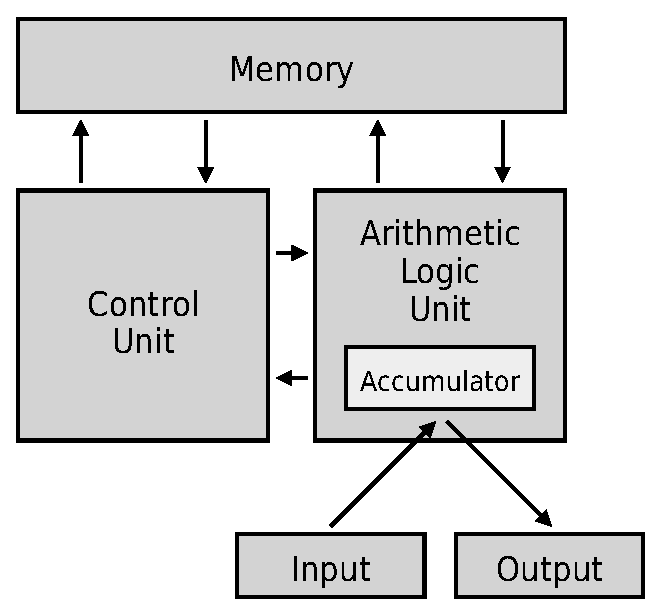
\includegraphics[width=0.6\textwidth]{Von_Neumann_architecture}
  \caption{Arquitectura Von Neumann}
\end{figure}
\subsection{Repertorio de instrucciones}

El funcionamiento del procesador está determinado por las instrucciones que ejecuta. Estas instrucciones se denominan \textit{instrucciones de maquina}. Al conjunto de instrucciones distintas quepuede ejecutar el procesador se denomina \textit{repertorio de instrucciones}.

\begin{subs}
  \subsubsection{Elementos de uns instrucciones de maquina}

  Cada instrucción debe contener la información que necesita el procesador para su ejecución. Dichos elementos son:

  \begin{itemize}
    \item \textbf{Código de operación}: especifica la operación a realizar (suma, E/S, etc.).
    \item \textbf{Referencia a operandos fuente u origen}: la operación puede implicar a uno o más operandos origen, es decir operandos que son entradas para la instrucción.
    \item \textbf{Referencia al operando de destino}: la operación puede producir un resultado que debe ser almacenado en un operando destino.
    \item \textbf{Referencia a la siguiente instrucción}: especifica la ubicación de la siguiente instrucción a ejecutar, (generamente la misma está implicita).
  \end{itemize}

  La siguiente instrucción a captar está en memoria principal o, en el caso de un sistema de memoria virtual, bien en memoria principal.
  Los operandos origen y destino pueden estar en alguna de las tres áreas siguientes:
  
  \begin{itemize}
    \item \textbf{Memoria principal o virtual}: como en las referencias a instrucciones siguientes, debe indicarse la dirección de memoria principal.
    \item \textbf{Registro del procesador}: un procesador contiene uno o más registros que pueden ser referenciados por instrucciones máquina.
    \item \textbf{Dispositivo de E/S}: la instrucción debe especificar el módulo y dispositivo de E/S para la operación. 
  \end{itemize}

  \begin{figure}[H]
    \centering
    \includegraphics[width=0.8\textwidth]{Ciclo-de-instruccion-CLI}
    \caption{Ciclo de instrucción}
  \end{figure}

  \subsubsection{Tipos de instrucciones}

  Cualquier programa escrito en alto nivel debe traducirse a lenguaje máquina para ser ejecutado. El repertorio de instrucciones máquina debe ser suficientemente amplio como para expresar cualquiera de las instrucciones e un lenguaje de alto nivel. Teniendo esto presente, los tipos de instrucciones se pueden clasificar de la siguiente manera:
  \begin{itemize}
    \item \textbf{Procesamiento de datos}: son instrucciones aritméticas y lógicas.
    \item \textbf{Almacenamiento de datos}: son instrucciones de memoria.
    \item \textbf{Transferencia de datos}: son instrucciones de E/S.
    \item \textbf{Control}: son instrucciones de comprobación y bifurcación.
  \end{itemize}

  Las instrucciones \textit{aritméticas} proporcionan capacidad computacional para procesar datos numéricos. Las instrucciones \textit{lógicas} operan con los bits de una palabra en lugar considerarlos como números. Las instrucciones \textit{memoria} permiten transferir los datos entre la memoria y los registros. Las instrucciones \textit{E/S} se necesitan para transferir programas y datos a memoria y devolver resultados de los cálculos al usuario. 

  \subsubsection{Número de direcciones}

  Una de las formas tradicionales de describir la arquitectura de un procesador es en términos del número de direcciones contenidas en cada instrucción. Esta dimensión se va haciendo menos significativa a medida que aumenta la complejidad del diseño del procesador.

  La mayoria de las instrucciones tienen una, dos o tre direcciones, estando implicita la dirección de la instrucción siguiente (obtenida a través del contador de programa)

  \begin{itemize}
    \item \textbf{Instrucciones de una dirección}: para funcionar, una segunda dirección debe estar implícita. La dirección implícita es el registro del procesador \textit{acumulador}. El acumulador contiene uno de los operandos y se emplea para almacenar el resultado.
    \item \textbf{Instrucciones de dos direcciones}: para operaciones binarias una de las direcciones debe hacer el servicio doble de uno de los operandos y del resultado. 
    \item \textbf{Instrucciones de tres direcciones}: no son comunes ta que requieren formatos relativamente largos para albergar las tres referencias. Una dirección es el destino y las otras dos son los operandos.
  \end{itemize}

  \subsubsection{Diseño del repertorio de instrucciones}

  El repertorio de instrucciones es el medio que tiene el programador para controlar el procesador. En consecuencia deben considerarse las necesidades del programador a la hora de diseñar el repertorio de instrucciones.

  Los aspectos fundamentales de diseño más importantes son:

  \begin{itemize}
    \item El \textbf{repertorio de operaciones}: cuántas y qué operaciones considerar, cuán complejas deben ser.
    \item Los \textbf{tipos de datos}: los distintos tipos de datos con los que se efectúan operaciones.
    \item Los \textbf{formatos de instrucciones}: longitud de la instrucción (en bits), número de direcciones, tamaño de los distintos campos, etc.
    \item Los \textbf{registros}: número de registros del procesador que pueden ser referenciados por las instrucciones, y su uso.
    \item El \textbf{direccionamiento}: el modo o modos de direccionamiento mediante los cuales puede especificarse la dirección de un operando.
  \end{itemize}

\end{subs}


\appendix

\section{Pilas}

Una \textbf{pila} es un conjunto ordenado de elementos, en el que solo uno de ellos es accesible en un instante dado. El punto de acceso se denomina \textit{cabecera} de la pila. El número de elementos en la pila, se denomina \textit{longitud}. Es una estructura de tipo \textit{LIFO} (Last In First Out), es decir, el último elemento en entrar es el primero en salir.

\begin{figure}[h]
  \centering
  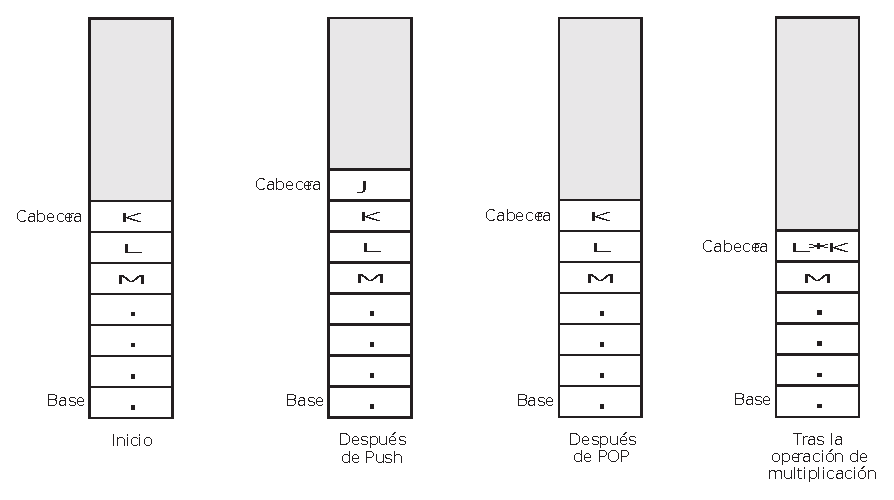
\includegraphics[width=0.8\textwidth]{Pila}
  \caption{Pila}
\end{figure}

La pila es una estructura útil como parte de la implementación del procesador. Por ejemplo, en el procesamiento de llamadas a subrutinas, la pila se utiliza para almacenar la dirección de retorno de la subrutina.

La implementación de una pila requiere que exista un cierto conjunto de posiciones utilizadas para almacenar los elementos de la pila.En memoria principal se reserva un bloque de posiciones contiguas para la pila.
Para un funcionamiento correcto se necesitan tres direcciones, normalmente memorizadas en registros del procesador:

\begin{itemize}
  \item \textbf{Stack pointer (SP)}: contiene la direccion del tope o cabecera de pila.
  \item \textbf{Stack base (SB)}: contiene la direccion de la base de la pila.
  \item \textbf{Stack limit (SL)}: contiene la direccion de la ultima posicion reservada de la pila.
\end{itemize}

\end{document}
